% cetal-slides-example.tex -- example deck for the draft CETAL Beamer theme
% Build:  latexmk -xelatex cetal-slides-example.tex   (LuaLaTeX also works)
\documentclass[aspectratio=169,11pt]{beamer}
\usetheme{CETAL}

\title[Example talk]{EMP amplitude scales with laser energy on target}
\subtitle{A worked example of the CETAL slide template}
\author[P.~Example]{\underline{Presenter Name}, Co-author Name}
\institute{CETAL, National Institute for Laser, Plasma and Radiation Physics (INFLPR), Măgurele, Romania}
\event{Group meeting}
\date{2026-10-14}

\cetalfunding{This work was supported by the Romanian Ministry of Research, Innovation and Digitalization
  through the INFLPR Core Programme LAPLAS~VII, contract 30N/2023.
  % TBC: confirm the project code with the Core Programme office before using it
}
\cetalcontact{presenter@inflpr.ro \quad\textperiodcentered\quad cetal.inflpr.ro}

\begin{document}

\begin{frame}[plain,noframenumbering]
  \titlepage
\end{frame}

\section{Results}

\begin{frame}{Peak field grows linearly with energy on all three probes}
  \begin{columns}[T]
    \begin{column}{0.52\textwidth}
      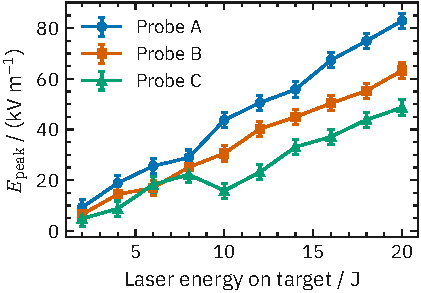
\includegraphics[width=\linewidth]{example-figure.pdf}
    \end{column}
    \begin{column}{0.44\textwidth}
      \begin{itemize}
        \item One message per slide, written as the title
        \item Figures made at final size, text close to the slide text
        \item Lines differ by marker as well as colour
        \item Units as quantity / unit: \(E\) / (kV\,m\(^{-1}\))
      \end{itemize}
    \end{column}
  \end{columns}
  \slidecite{Synthetic example data. Real sources: Author et al., \emph{Journal} \textbf{12}, 345 (2026).}
\end{frame}

\begin{frame}{Summary comes before the acknowledgements}
  \begin{enumerate}
    \item First conclusion, with its number
    \item Second conclusion
    \item What happens next
  \end{enumerate}
\end{frame}

\cetalclosingframe

\end{document}
